\documentclass{article}
\usepackage{graphicx}
\title{Torsional Axisymmetric Core Oscillations Visualiser} 
\author{Ogheneovo Mclarry Eduiyovwiri}
\date{August 5, 2020}
\begin{document}
\maketitle
\section{Introduction}
TACO-VIS provides a simple set of Python visualisation tools for 2D flow velocity data from fluid planetary interiors. It is mainly intended for animating torsional wave models for publication and presentation purposes. TACO-VIS is a lightweight module built only upon the common numpy/matplotlib Python packages and is free to be used and modified as the user requires.


\section{Dataset}

In this report we will be using this  software to write python script that produces the 3D animation of the Cox et al. (2013) azimuthal component of velocity, contour plots data to communicate the geometry of the waves within the spherical core.
It was meant to help visualize the spatially dependant modulating effect from the earth's magnetic field observations of which the torsional oscillations can constrain the strength of the magnetic field hidden deep inside the core.


\begin{figure}[h]
	    \centering
	        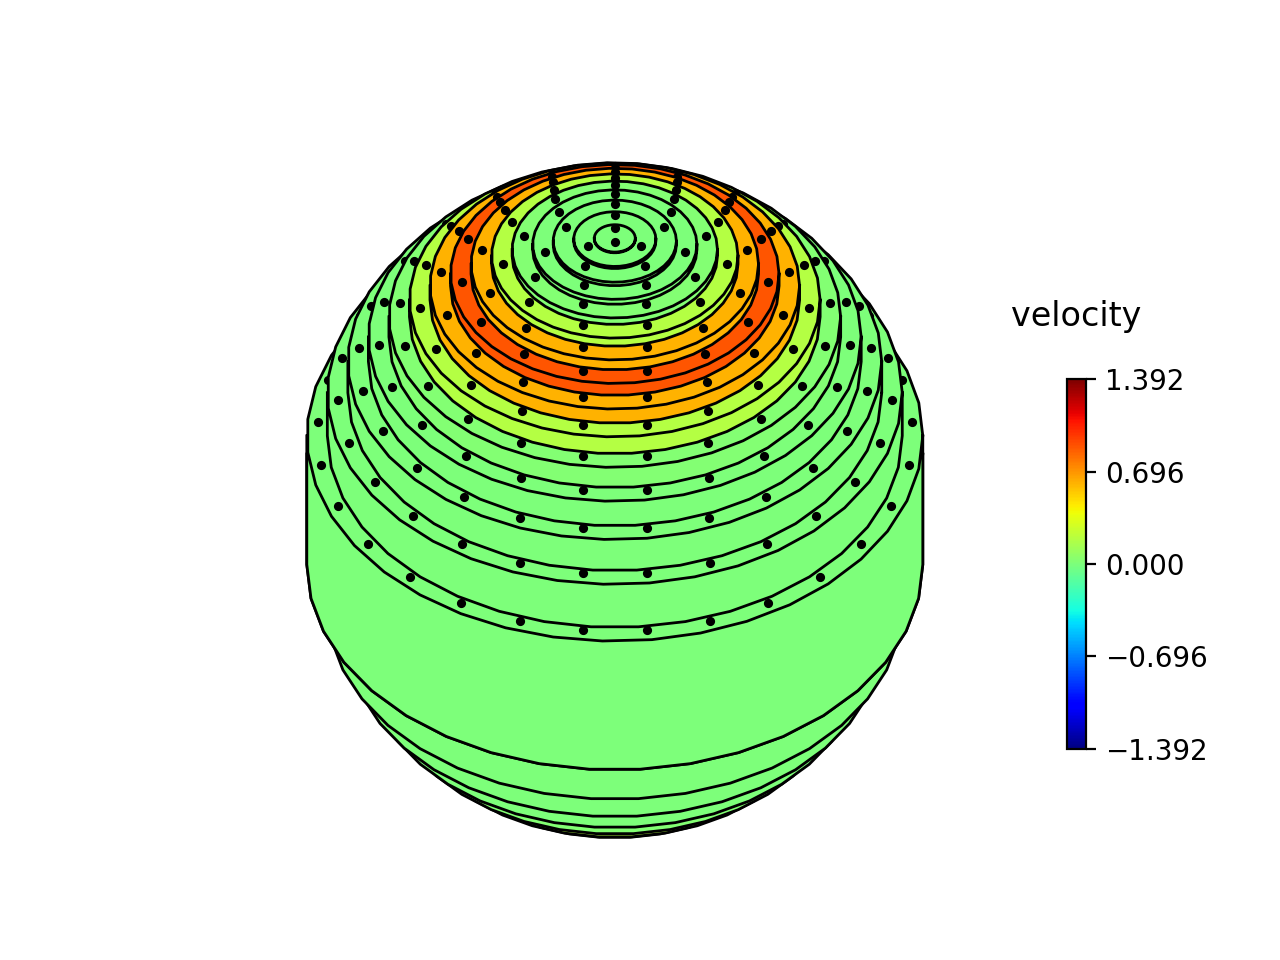
\includegraphics[width=0.5\textwidth]{myplot1.png}
		        \caption{A 3D and 2D visualisation of data from Cox et al. (Cox et al., 2013) approximated by 15 cylinders. The azimuthal velocity scale shown is non-dimensional and shared by both figures}
			    \label{fig:mesh1}
\end{figure}
 
 \section{Benefits of TACO-VIS include:}
 \begin{itemize}
	 \item .The tools require only the commonly available Python packages numpy and matplotlib and the well maintained ffmpeg framework.

	 \item .Generating an animation can be done in just a simple few lines of code, with examples provided.

	 \item .All plots and movies are of publication grade, with user choices for the titles, resolution and frame rate of saved images/movie files.
	 \item .The matplotlib animations often draw fast enough to be suitable to be viewed live (dataset depending) without the need to encode to a movie file first.

 \end{itemize}

\end{document}
